\documentclass[letterpaper]{article}

\usepackage{natbib,alifeconf}  %% The order is important


% *****************
%  Requirements:
% *****************
%
% - All pages sized consistently at 8.5 x 11 inches (US letter size).
% - PDF length <= 8 pages for full papers, <=2 pages for extended
%    abstracts.
% - Abstract length <= 250 words.
% - No visible crop marks.
% - Images at no greater than 300 dpi, scaled at 100%.
% - Embedded open type fonts only.
% - All layers flattened.
% - No attachments.
% - All desired links active in the files.

% Note that the PDF file must not exceed 5 MB if it is to be indexed
% by Google Scholar. Additional information about Google Scholar
% can be found here:
% http://www.google.com/intl/en/scholar/inclusion.html.


% If your system does not generate letter format documents by default,
% you can use the following workflow:
% latex example
% bibtex example
% latex example ; latex example
% dvips -o example.ps -t letterSize example.dvi
% ps2pdf example.ps example.pdf


% For pdflatex users:
% The alifeconf style file loads the "graphicx" package, and
% this may lead some users of pdflatex to experience problems.
% These can be fixed by editing the alifeconf.sty file to specify:
% \usepackage[pdftex]{graphicx}
%   instead of
% \usepackage{graphicx}.
% The PDF output generated by pdflatex should match the required
% specifications and obviously the dvips and ps2pdf steps become
% unnecessary.


% Note:  Some laser printers have a serious problem printing TeX
% output. The use of ps type I fonts should avoid this problem.


%\title{Ortus: Toward a Virtual Brain}
\title{Ortus: an Emotion--Driven Approach to (artificial) Biological Intelligence}
%\subpoint Ortus: an Emotion--Centric Approach to (artificial) Biological Intelligence
\author{Andrew W.E. McDonald, Sean Grimes,\and David Breen \\
\mbox{}\\
Drexel Unversity, Philadelphia, PA 19104 \\
awm32@cs.drexel.edu} % email of corresponding author

% For several authors from the same institution use the same number to
% refer to one address.
%
% If the names do not fit well on one line use
%         Author 1, Author 2 ... \\ {\Large\bf Author n} ...\\ ...
%
% If the title and author information do not fit in the area
% allocated, place \setlength\titlebox{<new height>} after the
% \documentclass line where <new height> is 2.25in



\begin{document}
\maketitle

\begin{abstract}
% Abstract length should not exceed 250 words
 Ortus is a simple virtual organism that also serves as a framework for developing biologically based artificial intelligence. Born from a goal to create complex virtual intelligence and an initial attempt to model C. elegans, Ortus implements a number of mechanisms observed in organic nervous systems, and attempts to fill in unknowns based upon plausible biological implementations, psychological observations. Implemented mechanisms include excitatory and inhibitory chemical synapses, bidirectional gap junctions, Hebbian learning with its Stentian extension.  We present an initial experiment that showcases Ortus'�� fundamental principles; specifically, a cyclic respiratory circuit, and emotionally--driven associative learning with respect to an input stimulus. Finally, we discuss the implications and future directions for Ortus and similar systems.


\end{abstract}

\section{Introduction}


While much work has been done to develop artificial intelligence (AI) systems that borrow principles from organic nervous systems, far less has been done that specifically targets the intersection of biology and artificial intelligence such that biological principles---rather than a specific applicability of the technology---are of primary concern, with the main goal being a virtual system that exhibits biological intelligence (BI). As our understanding of organic nervous systems and access to computation power both increase, widespread interest in systems that do exactly this is greatly increasing; as evidenced by DARPA's recent L2M project, in search of machines that learn throughout their lives \citep{darpa}.


Researchers in the realm of computational biology and neuroscience have started making progress toward developing systems that model specific organisms or neural circuits, such as the nematode Caenorhabditis elegans (C. elegans) \citep{Izquierdo2016}, though these systems have the potential to require too much focus on organism--specific details to achieve proper functionality, shifting focus away from creating more generalized neurologically--inspired intelligent systems.

On the other hand more traditional (application focused) AI research has started taking more inspiration from human learning, such as developing an auto--encoder augmented by Hebbian learning, decreasing the need for an initial supervised--like learning period \citep{Bowren2016}. Further, \citet{Marblestone2016} discusses ways that artificial neural networks (ANNs) can more closely approximate neural functionality.
In the context of biologically--inspired AI, the frameworks underlying these approaches may be too constraining for full exploration of the potential for that field of study. 

Recent work at the intersection of these two areas includes \citet{Sinapayen2016}, which investigates the applicability and biological plausibility of spiking neural networks learning by ``stimulation avoidance''. Perhaps the project most closely aligned to Ortus is a biologically inspired neural network modeled off of a honey bee's visual system, which merges biological mechanisms and neural networks \citep{Roper2017}.


\subsubsection{Ortus} is an initial implementation of, and framework for creating, virtual life aimed at approximating the intelligence of living organisms.
Bourn from the study and analysis of C. elegans' connectome and behavior, it aims to strike a balance between biological abstraction, retention of biological fidelity, and computation scalability in order to as closely as possible approximate biological intelligence and learning.
At its core, Ortus is a network of biologically--inspired, non--spiking neurons, capable of forming excitatory, inhibitory, and electrical synapses.
Similar to the way the structure of C. elegans' 302 neuron nervous system is capable of complex behaviors including toxin avoidance, reflexively withdrawing from a ``tap'', and ``remembering'' the temperature it found food  \citep{Jarrell2012}, Ortus' ``connectome'' (neural structure) enables its inherent functionality.
Once running, Ortus refines its network---similar to the way organic nervous systems adjust themselves, based upon Ortus' intrinsic ``understanding'' that certain things are ``good'' and others are ``bad'', with regard to its own longevity.
This understanding is derived from the structure of the nervous system it generates for itself from a set of input definitions given to it.


The remaining sections of this paper outline Ortus' design and implementation, describe an initial experiment, discuss the implications of this framework, and analyze its shortcomings.

\section{System Design}


As Ortus aims to be a virtual analogy to intelligent life, we tried to only implement functions that either had a known analogous biological process, or which may have an analogous biological implementation that is unknown, but can be defended based off anecdotal evidence. Following each Ortus design element (ODE) below, is its biological rationale (BR):

% 0: O2/CO2 respiratory framework, that provides a definition for emotional state 
% 1: emotion--driven
% 2: emotions tied to funcitonality necessary for life
% 3: sensory consolidatory inter neurons allow association of multiple stimuli with emotion (all emotions to each SCI..)
% 3: emotional backlink circuit to allow prior experiences connected to an emotional state to be recalled by that emotional state, if elevated (need not cross thresh..)
% 4: Hebbian learning (correlation), and Stentiann extension 
% 5: Ortus builds itself based off of rules, this creates a generally applicable/extensible framework 
% 7: certain emotional states dominate others
% 8: emotional interneurons connected via GJs to flood emotion through 'brain'
% 9: connection weights inverse to num connections

% somewhere in this section should be the diagram S => SEI => SCI

% do another diagram for actual network? probably not.

% diagram for respiratory circuit?

\textbf{ODE 1:} The underlying source of ``life'' for Ortus is its respiratory circuit, which maintains a balance of $O_2$ and $CO_2$. $O_2$ is consumed, and $CO_2$ is generated, as a product of Ortus being ``alive''. As $CO_2$ rises and $O_2$ falls, motor neurons responsible for excitation and inhibition of the lung muscle are excited and inhibited (respectively), and the lung increases in activation, supplying $O_2$ and expelling $CO_2$. 

\textbf{BR 1:} Maintaining a given system concentration of $CO_2$ is fundamental to mammalian life, and is very strongly linked to the mammalian fear response (e.g., you get scared if you can't breathe). The ability to regulate one's level of $CO_2$ appears to at least be part of the basis for defining what is a ``good'' and ``bad'' event/stimulus in the mammalian brain.

\textbf{ODE 2:} Currently, Ortus has two ``emotions'', fear and pleasure, represented by emotional interneurons, \texttt{eFEAR} and \texttt{ePLEASURE}, which are both tied into the respiratory circuit. When $CO_2$ rises, \texttt{eFEAR} rises, and Ortus would then be in a fearful state. As $CO_2$ falls, its contribution to Ortus' fearful state falls. The interaction between $O_2$ and \texttt{ePLEASURE} is the same. In this way, any stimulus presented in combination with either increased $CO_2$ or increased $O_2$ will become known as either a desirable (good) or undesirable (bad) stimulus. In this way, emotions are the driving force behind associative learning in Ortus. In Ortus, the idea of ``emotions'', are simply the rise and fall in activation of different neurons or groups of neurons, tied to very fundamental behaviors---such as ``breathing''. The concepts of ``good'' and ``bad'' sensations or emotions only carry meaning to us because of their associations to circuits that are either fundamentally desirable or undesirable from a longevity/survival perspective.

\textbf{BR 2:} Clearly, mammals don't normally get scared when they exhale, nor do they feel a measurable increase in pleasure upon inhalation, however the relations do exist on some level. As stated by \citet{Verma2015}, "emotions, motivations, and reinforcement are a closely related, evolutionarily---conserved phenomena maintaining the integrity of an individual and promoting survival in a natural environment". Along with \citet{Gore2015}, which suggests that associative learning is funneled through innate behavior circuits to assign positive or negative emotions to neutral sensory stimuli, it seems that building a virtual organism driven by emotional states is a fairly sound approach. 

While at the human level, the emotional ``part'' of the brain is quite complex, it is not unreasonable to assume that as organismic complexity (and thereby intelligence) decreases, the complexity of emotions decreases. Numerous experiments done on rodents, such as those described by \citet{Weiner2015}, show that the major structures of the brain can be examined by lesioning portions of the brain. One can infer then, that representing regions of the brain by single neurons would enable a rough approximation of the region's functionality. If one follows this line of thought, the possibility emerges that organisms like C. elegans may, in fact, be driven by ``emotions'' as well. For example, C. elegans is capable of toxin avoidance, a tap--withdrawal response, as well as learning that it found food at a certain temperature \textbf{(citations?)} -- one must ask how this can be. There is nothing external that assists it in differentiating good from bad, yet it wants to avoid certain things, while is attracted to others. In Ortus, we make the assumption that that these behaviors are a result of a \textit{very} simple emotional subsystem that forms the basis for C. elegans' behavior.


\textbf{ODE 3:} Ortus employs four different classes of interneurons at the moment. First are ``Sensory Extension Interneurons'' (SEIs). These take input directly from sensory neurons, and pass the input along to the second class of interneurons, ``Sensory Consolidatory Interneurons'' (SCIs).
SCIs take anywhere from 1 to the number of sensory inputs as chemical synapses, with incoming synaptic weights equal to \textit{1 / (\# sensory inputs)}.
The idea behind SCIs is to enable different types of sensors to combine their input, and trigger emotions, effectively as a ``new'' sensory input, thereby forming associations between two stimuli. We defer the descriptions of the last two interneurons to \textbf{ODE 5}.

\textbf{BR 3:} Admittedly, SEIs may not be necessary. We included these so that we could give sensory neurons a functionality that was separate from interneurons if the need arose. With regard to SCIs, it is suggested by \citet{Xie2016} that neurons in the brain are organized according to the idea that if there are $N$ neurons, then the brain has the ability to represent all $2^N-1$ possible combinations. Clearly, for anything but the most simple organisms, having one neuron that collects the input for each of the $2^N-1$ possibilities is unrealistic (as the authors note); however, the authors suggest there may be additional combining of neuron inputs to decrease the computational and spacial complexity (in organic brains, that is). It also possible that mammalian brains are not quite as connected as their owners are led to believe, and a great deal of what amounts to interpolation is the reality. Regardless, we employed the idea of $2^N-1$ SCIs because losing sensory resolution with such few neurons (that only have one neuron per sensory input) doesn't make sense. This will have to be reassessed. There is, however, a far stronger argument for the strength of the SCI inputs: it seems that synaptic strength scales inversely with the number of connections, ``$K$ as ~ $1 \over \sqrt{k}$'' \citep{Barral2016}. This makes intuitive sense; if neuron \texttt{A} synapses onto \texttt{B} with a weight of $1$, and \texttt{C, D, E} all synapse onto \texttt{F}, the weight of each of the latter three connections must be $1 \over 3$ in order to maintain equivalence between \texttt{B} and \texttt{F}. In addition, there is evidence that neighboring neurons in the same ``layer'' are connected in C. elegans \citep{Azulay2016}, which suggests that a certain amount of information consolidation may occur.


\textbf{ODE 4:} Ortus currently implements both Hebbian learning and the Stentian extension to Hebbian learning. Specifically, for each chemical synapse, on every timestep, if activity is sufficiently synchronous or sufficiently asynchronous, the synapse strengthens or weakens (respectively) according to its \textit{mutability index} (\textit{MI}). The \textit{MI} determines a synapses' potential to be modified. Currently, \textit{MI}s are static, though in the future we plan to vary them with synaptic age, among other things.

\textbf{BR 4:} Hebbian and Stentian learning, relating to the correlation (or lack thereof) between presynaptic and postsynaptic pairs is a proven learning paradigm in neuroscience, as described by \citet{Kutsarova2016}.



\textbf{ODE 5:} The third class of interneurons is comprised of ``Emotion Extension Interneurons'' (EEIs), which are essentially auxiliary emotion neurons.
EEIs are specific to each emotion, and receive input from SCIs via chemical synapses, and pass that input on to their respective primary emotion neurons via gap junctions.
Emotional learning is achieved by strengthening synapses (via Hebbian learning) of interneurons that form synapses between SCIs (consolidated sensory information), and EEIs.
The GJ connection enables a given emotional state, incurred by any stimulus, to permeate through Ortus---resulting in an ``emotional state'' of the system (gap junctions in Ortus have no activation threshold).
The effect of this, is that if a certain sensory input causes a given emotion to increase in activation, the introduction of another sensory input will cause the synapses at the junction of the newly introduced sensory input and elevated emotion to strengthen. (graph here?). 
Further, as each SCI synapses onto one EEI per emotional state, each EEI has a ``backlink'' chemical synapses to their parent SCI.
The idea behind the backlinks is to allow an emotional state to ``trigger'', or cause Ortus to ``remember'' a stimulus that previously invoked (and thus become associated with) that emotional state.
In this case, ``remembering'' is defined as measurably increased activation in the SCI that the EEI backlinks into.
In practice, we have observed a very slight difference in Ortus as a result of the backlink connections; currently they exist more as a concept that doesn't break the system. A diagram of this layout may be seen in \textbf{DIAGRAM!}.

\textbf{BR 5:} Specifically with regard to the mammalian dopamine circuit, there exists a small locus of dopaminergic cells, but the they receive inputs from diverse sources, as well as project to divers parts of the brain, as discussed by \citet{Beier2015}. From a psychological perspective, it is clear that when one enters an emotional state, the emotion is encompassing, not localized. It is also clear that a stimulus or activity is likley to be ``colored'' by the emotional state one was in when the stimulus occurred. The approach we took with Ortus is a simplification of the dopamine circuit, and a generalization across emotional states; it will likely need refinement.

\textbf{ODE 6:} Certain emotional states preside over (dominate) others. In Ortus, fear dominates pleasure.

\textbf{BR 6:} The idea of a hierarchical system, where certain emotional states dominate others, is supported by the inhibition of fear in mice, in favor of searching for food when hungry (blood glucose levels falling causing the release of hormones), but greater concern for safety when not hungry \citep{Verma2015}. Further, \citet{Leknes2008} discusses the ``Motivation--Decision Model'', which suggests that anything that is more important for survival than pain should inhibit the feeling of pain.



\textbf{ODE 7:} Ortus builds its nervous system by reading in a \textit{.ort} file, using our ``\textit{Ortus Development Rules}'' language. First, ``elements'' (neurons and muscles) must be specified, with attributes such as the type of element, its affect, and activation threshold. Then, relationships between elements may be specified. Currently, there are four relationships:
\begin{itemize}
    \itemsep0em
   \item \texttt{+A} \textbf{causes} \texttt{+B}
        \subitem Where the ``+'' indicates an increase (and a ``-'' a decrease) in the presynaptic neuron causes an increase in the postsynaptic neuron. This translates into a chemical synapse.
    \item \texttt{A} \textbf{correlated} \texttt{B}
        \subitem Where A and B are correlated. This translates into a gap junction.
    \item \texttt{A} \textbf{opposes} \texttt{B}
        \subitem Where A and B inhibit each other.
     \item \texttt{A} \textbf{dominates} \texttt{B}
         \subitem Where A inhibits B.
\end{itemize}

Along with relationship--level attributes such as: ``mutability'', ``weight'', ``polarity'', and ``age''. At this time, most relationship attributes need not be specified as Ortus uses default values. Once Ortus reads these instructions in, it creates interneurons and connections as described by the \textbf{ODE}s above to satisfy all constraints imposed, and to allow associative learning between all emotional states and sensory stimuli (both individual and combined) as described in \textbf{ODE 5}.


\textbf{BR 7:}

Our goal in creating the \textit{Ortus Development Rules} was to approximate, in a greatly simplified manner, the way a brain grows itself, based upon genetic instructions that cause circuits to form in certain ways via gene expression \citep{Weiner2015}. Ortus' neural structure is essentially wired to force it to behave in certain ways, similarly to the development of the mammals, and how genes . Further, \citet{Schroter2017} provides evidence for the existence of organizational ``motifs'' found in C. elegans that may underly more complex networks in larger brains; this also lends credence to Ortus' rule--based development approach.


%the ORT filetype is a specification of ``rules'', akin to very simplified approximation ``virtual DNA'' that define elements (neurons and muscles), and relationships between them, currently: A causes B, A is correlated with B, A opposes B, and A dominates B. Each realtionship has a number of paramters, such as Age, Mutability, Threshold, and either a chemical synapse (CS) weight (unidirectional), or a gap junction (GJ) weight (bidirectional) (NOTE: equations!).



%\begin{enumerate}
%    \item \textbf{element:} \texttt{sO2: \{type=sense, affect=pos\}}
%    \item \textbf{element:} \texttt{sCO2: \{type=sense, affect=neg\}}
%    \item \textbf{element:} \texttt{eFEAR: \{type=emotion, affect=neg\}}
%    \item \textbf{element:} \texttt{ePLEASURE: \{type=emotion, affect=pos\}}
%    \item \textbf{element:} \texttt{mINHALE: \{type=motor\}}
%    \item \textbf{element:} \texttt{mEXHALE: \{type=motor\}}
%    \item \textbf{element:} \texttt{LUNG: \{type=muscle\}}
%    \item \texttt{sO2} \textbf{opposes} \texttt{sCO2}
%    \item \texttt{mINHALE} \textbf{opposes} \texttt{sCO2}
%    \item \texttt{+A} \textbf{causes} \texttt{+B}
%    \item \texttt{A} \textbf{dominates} \texttt{B}
%\end{enumerate}<++>


\subsection{Implementation Details} Ortus is written in C++ and OpenCL. Each iteration of the OpenCL kernel constitutes one timestep, during which, each neuron sums incoming (positive or negative) ``activation'' from presynaptic cells via chemical synapses (CSes) and gap junctions (GJs).  \textbf{NOTE: maybe this is a good spot for the equations!}

The chemical synapse and gap junction activation transfer equations were simplified from those described by \cite{Wicks1996} to ignore physical properties of neurons (such as neuron length).

Ortus' neurons are based upon C. elegans' neurons, and are non--spiking, but do not transmit any ``activation'' (footnote about why activation is used instead of voltage? or use 'potential?) below a given threshold, as in \citep{Graubard1014}. The equations for CS and GJ synapses were derived (simplified) from Wicks' 1996 paper (cite), and appear to have been used in recent C. elegans' models (cite Beer's 2013).


% CS equation

% GJ equation

% voltage leak

% 


\subsubsection{Implementation Details}
- C++, OpenCL
- each neuron operates on its incoming connections, so it only does ``postsynaptic'' work, leaving its ``presynaptic'' work to neurons that it is presynaptic to (see ``shortcomings'')
- sensory consolidation causes resolution loss, currently maximum resolution for any sensor array (e.g., not just O2) has a maximum resolution of 2 for intra--sensor consolidation, and 3 for inter--sensor consolidation. Single neuron sensors have no minimum for either. (NOTE: sensor array not implemented yet... take this out if it doesn't get implemented)

\section{Experimental Design and Results}

\subsubsection{Experiment.} To test our initial implementation of Ortus, we implemented the configuration described above, with the addition of an $H_2O$ sensory neuron. We then ``exposed'' Ortus to water via $H_2O$ sensory stimulation four times in bursts spaced 100 timesteps apart, in order to allow injected activation to naturally decay. During each burst of $H_2O$ exposure, we prevented Ortus from exhaling $CO_2$ or inhaling $O_2$, thereby inducing an enhanced state of fear. After repeating the conditioning exposure four times, we allowed Ortus 200 timesteps to let any injected activation to decay. Finally, we exposed Ortus to water, without inducing a fearful state, to determine if it had learned to be fearful of water.

\subsubsection{Results.} Since $CO_2$ activation causes fear, and $H_2O$ was presented during this time, we expected Ortus to become progressively more and more ``scared'' of water each time it was presented while it was in a state of elevated fear. As can be seen in \textbf{FIGURE}, during each exposure to $H_2O$, activation of \texttt{eFEAR} increased when compared to the previous exposure. Further, after the four rounds of conditioning, we observed a large spike in fear. Compared to simply exposing Ortus to $H_2O$ without prior fear conditioning, in which a very slight raise was observed, it is clear that we were able to successfully use classical conditioning to instill a fear of water in Ortus that was previously almost non--existent. 

\ldots. should probably show graph of what happens when O2 isn't inhibited\ldots


\section{Discussion}
While the implementation presented is quite simple, the initial results presented pave the way for quick advances to Ortus' capability with regard to ``behaviors'' resulting from emotional amalgamation as well as the introduction of more complex sensory input.


Clearly more emotions can be added, and can be combined in various ways, meaning there is the potential for Ortus to experience quite complex emotional states.

While Ortus' eventual goal is to develop complex ``neural'' functionality akin to that observed in complex systems, we

\citet{Kutsarova2016} indicates that, relative to synaptic strengthening and weakening, axonal branch tips emerge to form new synapses. synchronous activity stabilizes synapses and prolongs axonal branches. This is one way for Ortus to alter its structure in addition to synaptic weights.

\cite{Johansens2014} suggests that in mice, while synchronous activity (correlation) is necessary for synaptic plasticity, it is not sufficient; neuromodulatory signaling is also required. This could be a way to control some of the unstable behavior seen as a result of the purely correlation--based learning rules implemented.


Since disabling different parts of a given circuit can have slightly different effects (e.g. males will seek males, instead of females) \citet{Weiner2015}, it should be feasible to grow portions of Ortus where more nuanced behavior is desired.

However one current issue is if we have SCIs for sensory neurons \texttt{A}, and \texttt{B}, we will have \texttt{iA}, and \texttt{iB}, and \texttt{iAB}. If \texttt{iAB} is activated, that means that \texttt{iA} and \texttt{iB} will also be activated. A solution might be for more complex SCIs to inhibit less complex ones, though that would perhaps unnecessarily add to computational complexity.

Sensory stimulation is sensed by sensory neurons that are topographically arranged, similar to those in organic systems. A recent study suggesting that the brain is organized based upon an n = 2something... and something about permutations lends credence to this approach (cite n something 2 permutation paper).


Talk about the combinatorial explosion, but then discuss how that can be pruned away... similar to babies. The $2^n - 1$ paper suggested reducing the resolution of inputs, so, instead of each sensor being able to connect with every other sensor, funnel 3 sensors (for example) into 1, to create a ``functional connectivity module'' (FCM). That approach might not be bad, however, it could be severely limiting. Perhaps this can be cut down by looking at relationships between sensors, and getting rid of things that don't matter?

Choices are:
1) an array of 9 sensors, if 0,1,2 > A, 2,3,4 > B, 4,5,6 > C, 6,7,8 > D, then sum {nCr(k,n)} for n from 1 to k is $2^n - 1$. It is clear that to get a fully connected network, capable of expressing all possible combinations, even from a living organism perspective, things become unfeasible.

2) Rather, it is probably the case that our brains aren't quite as connected as they appear to be. (e.g., within a certain radius, two places on your skin feel like the same location. visual system either might be an exception, however it is well known that visual information gets interpolated.)
There must be some sort of neural processing shortcuts ... approximation. e.g., if you are quickly reading, you might read "New York", when the only word there was "York"



\cite{Weiner2015} talks about topographic organization\ldots useful for sensors in array (e.g. visual)

Need to implement habituation 

From an artificial intelligence standpoint, the

\begin{enumerate}
\item less connections
\item ability to specify initial behavior
\item don't need a massive training set
\item 3 types of interactions: inhibitory CS, excitatory CS, and GJ.
\end{enumerate}

Together, these afford artificial neural networks far greater flexibility and thereby power. It is possible that this will enable more nuanced behavior.

From an artificial life standpoint: people are modeling networks with less complexity than this to attempt to recreate C. elegans' behavior from its connectome (cite openworm). This work pivoted from that approach, because in attempting to model the entire connectome, it became clear that there were too many unknowns. However, it also became clear that there was a certain logic to the way the neurons were wired; a notion backed up by (cite c elegans wiring works... have some in mendeley).

A simple idea is, how can C. elegans <DO SOMETHING> -- point here is to describe the requirement that certain things inhibit while others excite, in order to allow a certain behavior to happen.



\citet{Schroter2017} suggests that C. elegans' neurons may have multiplexed functions, meaning that one neuron may contribute to more than one behavior. This is another possible way to decrease the number of necessary neurons in Ortus.


floor so that learned stuff can't be unlearned beyond a certain point -- e.g., as a relationship ages, it's mutability should tend toward 0.


\subsubsection{Shortcomings and Issues.}
There is no temporal differentiation between CS and GJ transmission. On each timestep, neurons collect all incoming ``activation'' from.

There is minimal presynaptic processing -- (NOTE:how true is this? )

No location--based axon growth, as is seen in, relative to hebbian plasticity (cite)





\section{Conclusion}
We have presented Ortus, an initial approach to a framework that exhibits basic emotionally--based learning (fear conditioning), self--sustaining inherent behavior (cyclic breathing), and a topographical approach to sensory processing that enables inter-sensory associative learning, with or without an emotional component.

Ortus also has a system to map sensory inputs such as "breathe" to the stimulation of O2 sensors.






\section{Acknowledgements}

This work was supported by NSF grant No.\ ?????????????????.

\footnotesize
\bibliographystyle{apalike}
\bibliography{ortus_paper} % replace by the name of your .bib file


%\section{Self-Organization in Evolution}
%
%The idea that the evolutionary process occurs in spurts, jumps, and
%bursts rather than gradual, slow and continuous changes has been
%around for over 75 years \citep{WIL}, but has gained prominence as
%``punctuated equilibrium'' through the work of \citet{GE77,GE93}. The
%general idea is that evolutionary innovations are not bestowed upon an
%existing species as a whole, gradually, but rather by the emergence of
%{\em one} better adapted mutant which, by its superiority, serves as
%the seed of a new breed that sweeps through an ecological niche and
%supplants the species previously occupying it. The global dynamics
%thus has a microscopic origin, as shown experimentally, e.g., in
%populations of {\it E. Coli} \citep{ECL96}.
%
%Such avalanches can be viewed in two apparently contradictory ways. On
%the one hand we may consider the wave of extinction touching all
%species that are connected by their ecological relations, a process
%akin to percolation and therefore suitably described by the language
%of second-order critical phenomena \citep{BS}. Such a scenario relies
%on the {\em coevolution} of species (to build their ecological
%relations) and successfully describes power-law distributions obtained
%from the fossil record \citep{SB96,BP96}. There is, on the other hand,
%a description in terms of {\em informational} avalanches that does not
%require coevolution and leads to the same statistics, as we show
%here. Rather than contradicting the aforementioned picture
%\citep{NFST}, we believe it to be complementary.
%
%In the following, we set up a scenario in which {\em information} is
%viewed as the agent of self-organization in evolving and adapting
%populations. Information is, in the strict sense of Shannon theory, a
%measure of correlation between two ensembles: here a population of
%genomes and the environment it is adapting to. As described elsewhere
%\citep{IAL}, this correlation grows as the population stores more and
%more information about the environment via random measurements,
%implementing a very effective {\em natural Maxwell demon}. Any time a
%stochastic event increases the information stored in the population, a
%wave of extinction removes the less adapted genomes and establishes a
%new era. Yet, information cannot leave the population as a whole,
%which therefore may be thought of as protected by a {\em
%semi-permeable membrane} for information, the hallmark of the Maxwell
%demon. Let us consider this dynamics in more detail.
%
%The simple living systems we consider here are populations of
%self-replicating strings of instructions, coded in an alphabet of
%dimension ${\cal D}$ with variable string length $\ell$. The total
%number of possible strings is exponentially large. Here, we consider
%the subset of all strings currently in existence in a finite
%population of size $N$, harboring $N_g$ different types, where
%$N_g\ll{\cal D}^\ell$. Each {\em genotype} (particular sequence of
%instructions) is characterized by its replication rate $\epsilon_i$,
%which depends on the sequence only, while its survival rate is given
%by $\epsilon_i/\langle \epsilon\rangle$, in a ``stirred-reactor''
%environment that allows a mean-field picture. This average replication
%rate $\langle \epsilon\rangle$ characterizes the fitness of the
%population as a whole, and is given by
%\begin{eqnarray}
%\langle \epsilon\rangle=\sum_i^{N_g}\frac{n_i}N \epsilon_i\;,
%\end{eqnarray}
%where $n_i$ is the {\em occupation number}, or frequency, of genotype
%$i$ in the population. As $N_g$ is not fixed in time, the average
%depends on time also, and is to be taken over all genotypes currently
%living. The total abundance, or size, of a genotype is then
%\begin{eqnarray}
%s_i=\int_0^\infty n_i(t)\, dt=\int_{T_c}^{T_e}n_i(t)\, dt\;,
%\label{size}
%\end{eqnarray}
%where $T_c$ is the time of creation of this particular genotype, and
%$T_e$ the moment of extinction. Before we obtain this distribution in
%Avida, let us delve further into the statistical description of the
%extinction events.
%
%At any point in time, the fate of every string in the population is
%determined by the craftiness of the best adapted member of the
%population, described by $\epsilon_{\rm best}$. In this simple,
%finite, world, which does not permit strings to affect other members
%of the population except by replacing them, not being the best reduces
%a string to an ephemeral existence. Thus, every string is
%characterized by a {\em relative} fitness, or {\em inferiority}
%\begin{eqnarray}
%E_i=\epsilon_{\rm best}-\epsilon_i
%\end{eqnarray}
%which plays the role of an {\em energy} variable for strings of
%information {IAL}. Naturally, $\langle E\rangle=0$ characterizes the
%{\em ground state}, or vacuum, of the population, and strings with
%$E_i>0$ can be viewed as occupying {\em excited} states, soon to
%``decay'' to the ground state (by being replaced by a string with
%vanishing inferiority). Through such processes, the dynamics of the
%system tend to minimize the average inferiority of the population, and
%the fitness landscape of replication rates thus provides a Lyapunov
%function. Consequently, we are allowed to proceed with our statistical
%analysis. Imagine a population in equilibrium, at minimal average
%inferiority as allowed by the ``temperature'': the rate (or more
%precisely, the probability) of mutation. Imagine further that a
%mutation event produces a new genotype, fitter than the others,
%exploiting the environment in novel ways, replicating faster than all
%the others. It is thus endowed with a new best replication rate,
%$\epsilon_{\rm best}^{\rm new}$, larger than the old ``best'' by an
%amount $\Delta \epsilon$, and redefining what it means to be
%inferior. Indeed, all inferiorities must now be {\em renormalized}:
%what passed as a ground state ($E=0$) string before now suddenly finds
%itself in an excited state. The seed of a new generation has been
%sown, a phase transition must occur. In the picture just described,
%this is a first-order phase transition with latent heat
%$\Delta\epsilon$ (see Fig.\ref{fig1}), starting at the ``nucleation''
%point, and leading to an expanding {\em bubble} of ``new phase''.
%
%
%\begin{figure}[t]
%\begin{center}
%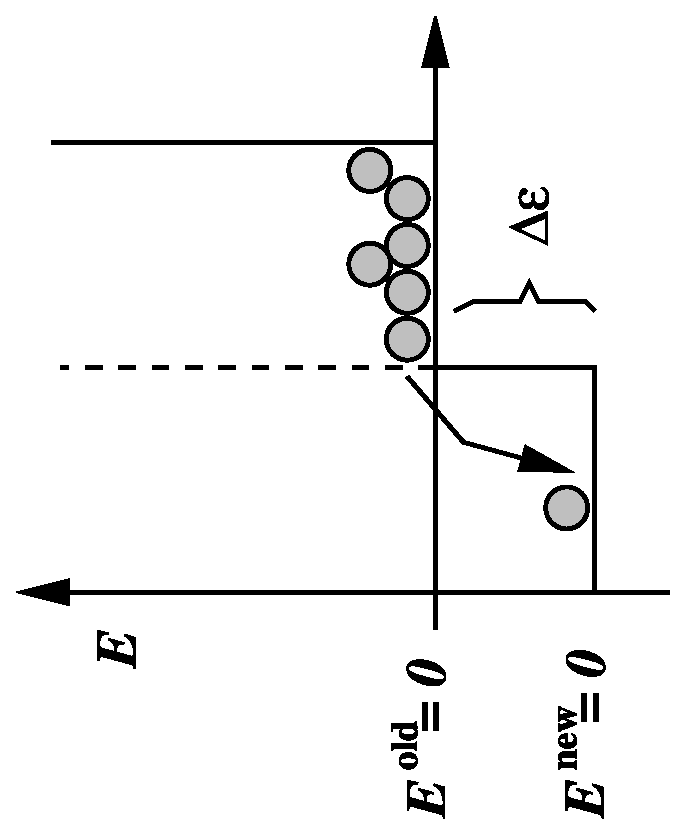
\includegraphics[width=2.1in,angle=-90]{fig1.eps}
%\caption{``Energies'' (inferiorities) of strings in a first-order
%  phase transition with latent heat $\Delta\epsilon$.}
%\label{fig1}
%\end{center}
%\end{figure}
%
%This bubble expands with a speed given by the Fisher velocity
%\begin{eqnarray}
%v\sim\sqrt{D\Delta\epsilon}\;, \label{eq4}
%\end{eqnarray}
%where $D$ is the diffusion coefficient (of information) in this
%medium, until the entire population has been converted \citep{CHU}.
%This marks the end of the phase transition, as the population returns
%to equilibrium via mutations acting on the new species, creating new
%diversity and restoring the {\em entropy} of the population to its
%previous value. This prepares the stage for a new avalanche, as only
%an equilibrated population is vulnerable to even the smallest
%perturbation. The system has returned to a critical point, driven by
%mutations, self-organized by information.
%
%Thus we see how a first-order scenario, without coevolution, can lead
%to self-organized and critical dynamics. It takes place within a
%single, finite, ecological niche, and thus does not contradict the
%dynamics taking place for populations that span many niches. Rather,
%we must conclude that the descriptions complement each other, from the
%single-niche level to the ecological web. Let us now take a closer
%look at the statistics of avalanches in this model, i.e., at the
%distribution of genotype sizes.
%
%
%\section{Exponents and Power Laws}
%
%\hyphenation{ap-proximated}
%
%In this particular system avalanche size can be approximated
%by the size $s$ of the genotype that gave rise to it,
%Eq.~(\ref{size}).  We shall measure the distribution of these sizes
%$P(s)$ in the Artificial Life system Avida, which implements a
%population of self-replicating computer programs written in a simple
%machine language-like instruction set of ${\cal D}=24$ instructions,
%with programs of varying sequence length. In the course of
%self-replication, these programs produce mutant off-spring because the
%{\tt copy} instruction they use is flawed at a rate $R$ errors per
%instruction copied, and adapt to an environment in which the
%performance of {\em logical} computations on externally provided
%numbers is akin to the catalysis of chemical reactions \citep{OBA}. In
%this {\em artificial chemistry} therefore, successful computations
%accelerate the metabolism (i.e., the CPU) of those strings that carry
%the {\em gene} (code) necessary to perform the trick, and any program
%discovering a new trick is the seed of another avalanche.
%
%Avida is not a stirred-reactor environment (although one can be
%simulated). Rather, the programs live on a two-dimensional grid, each
%program occupying one site. The size of the grid is finite, and chosen
%in these experiments to be small enough that avalanches are generally
%over before a new one starts. As is well-known, this is the condition
%{\em sine qua non} for the observation of SOC behavior, a separation
%of time scales which implies that the system is driven at
%infinitesimal rates.
%
%Let $\tau$ denote the average duration of an avalanche. Then, a
%separation of time scales occurs if the average time between the
%production of new seeds of avalanches is much larger than $\tau$. New
%seeds, in turn, are produced with a frequency $\langle\epsilon\rangle
%P$, where $\langle\epsilon\rangle$ is again the average replication
%rate, and $P$ is the mutation probability (per replication period) for
%an average sequence of length $\ell$,
%\begin{eqnarray}
%P=1-(1-R)^\ell\;.
%\end{eqnarray}
%For small enough $R$ and not too large $\ell$ (so that the product
%$R\ell$ is smaller than unity) we can approximate
%$P\approx R\ell$, and infinitesimal driving occurs in the limit
%\begin{eqnarray}
%\langle \epsilon\rangle R\ell \ll\frac1\tau\;.\label{cond}
%\end{eqnarray}
%Furthermore
%\begin{eqnarray}
%\tau\sim\frac{L}v
%\end{eqnarray}
%with $L$ the diameter of the system and $v$ a typical Fisher velocity.
%The fastest waves are those for which the latent heat is of the order
%of the new fitness, i.e., $\Delta\epsilon\sim\epsilon$, in which case
%$v\approx \epsilon$ \citep[because $D\sim\epsilon$ in
%Eq.~(\ref{eq4}),][]{CHU}, and a separation of time scales is assured
%whenever
%\begin{eqnarray}
%\frac1{R\ell}\gg {L}\;,
%\end{eqnarray}
%that is, in the limit of vanishing mutation rate or small population
%sizes. For the $L=60$ system used here, this condition is obeyed (for
%the fastest waves) only for the smallest mutation rate tested and
%sequence lengths of the order of the ancestor.
%
%
%\begin{figure}[t]
%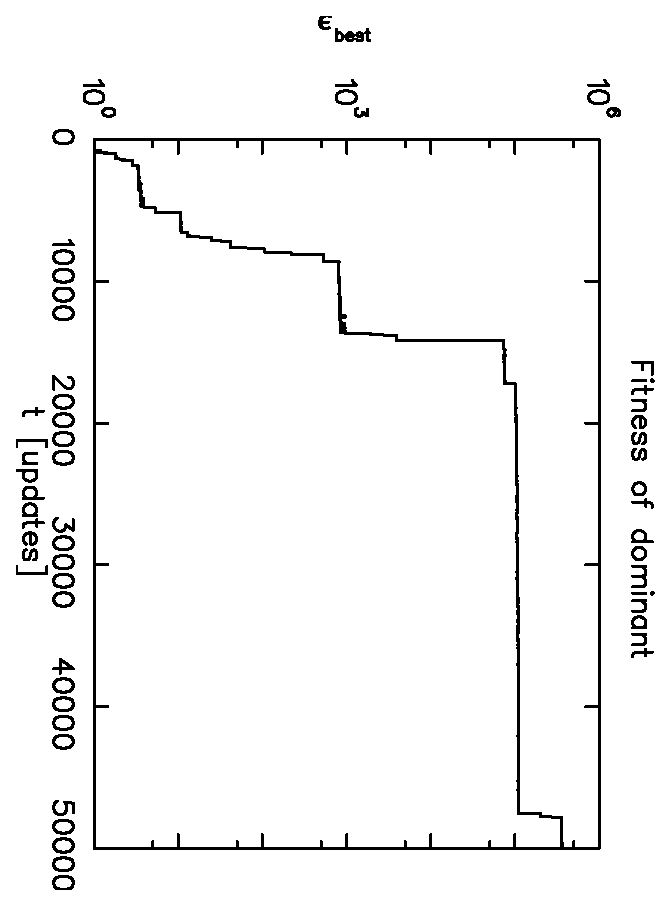
\includegraphics[width=2.3in, angle=90]{fig2.eps}
%\caption{Fitness of the dominant genotype in the population, $\epsilon_{\rm best}$ as a function of time (in updates).}
%\label{fig2}
%\end{figure}
%
%
%In the following, we keep the population size constant (a $60\times60$
%grid) and vary the mutation rate. From the previous arguments, we
%expect true scale-free dynamics only to appear in the limit of small
%mutation rates.  As in this limit avalanches occur less and less
%frequently, this is also the limit where data are increasingly
%difficult to obtain, and other finite size effects can come into play.
%We shall try to isolate the scale-free regime by fitting the
%distribution to a power law
%\begin{eqnarray}
%P(s)\sim s^{-D(R)}\label{power}
%\end{eqnarray}
%and monitor the behavior of $D$ from low to high mutation rates.
%
%In Fig.~\ref{fig2}, we display a typical history of $\epsilon_{\rm
%best}$, i.e., the fitness of the dominant genotype.\footnote{As the
%replication rate $\epsilon$ is exponential in the bonus obtained for a
%successful computation, $\epsilon_{\rm best}$ increases exponentially
%with time.}  Note the ``staircase'' structure of the curve reflecting
%the ``punctuated'' dynamics, where each step reflects a new avalanche
%and concurrently an extinction event. Staircases very much like these
%are also observed in adapting populations of {\it E. Coli}
%\citep{LT94}.
%
%As touched upon earlier, the Avida world represents an environment
%replete with information, which we encode by providing bonuses for
%performing logical computations on externally provided (random)
%numbers. The computations rewarded usually involve two inputs $A$ and
%$B$, are finite in number and listed in Table~1. At the end of a
%typical run (such as Fig.~\ref{fig2}) the population of programs is
%usually proficient in almost all tasks for which bonuses are given
%out, and the genome length has grown to several multiples of the
%initial size to accommodate the acquired information.
%
%\begin{table}[h]
%\center{
%\begin{tabular}{|c|c|c|c|}\hline
%Name & Result & Bonus $b_i$ & Difficulty\\ \hline\hline
%Echo & I/O   & 1 & --\\
%Not  & $\neg A$ & 2 & 1 \\
%Nand & $\neg(A\wedge B)$ & 2 & 1 \\
%Not Or & $\neg A \vee B$ & 3 & 2 \\
%And  &  $ A \wedge B $   & 3 & 2 \\
%Or   &  $ A \vee B $     & 4 & 3 \\
%And Not & $A\wedge\neg B$& 4 & 3 \\
%Nor  & $\neg(A\vee B)$   & 5 & 4 \\
%Xor  & $ A\ {\rm xor}\ B$ &   6 & 4 \\
%Equals &$\neg(A\ {\rm xor}\ B)$&6& 4 \\ \hline
%\end{tabular}
%}
%\vskip 0.25cm
%\caption{Logical calculations on random inputs $A$ and $B$ rewarded,
%bonuses, and difficulty (in minimum number of {\tt nand} instructions
%required). Bonuses $b_i$ increase the speed of a CPU by a factor
%$\nu_i=1+2^{b_i-3}$.}
%\end{table}
%
%Because the amount of information stored in the landscape is finite,
%adaptation, and the associated avalanches, must stop when the
%population has exhausted the landscape.  However, we shall see that
%even a `flat' landscape (on which evolution is essentially neutral
%after the sequence has optimized its replicative strategy) gives rise
%to a power law of genotype sizes, as long as the programs do not
%harbor an excessive amount of ``junk'' instructions.  A typical
%abundance distribution (for the run depicted in Fig.~\ref{fig2}) is
%shown in Fig.~\ref{fig3}.
%
%
%\begin{figure}[ht]
%\begin{center}
%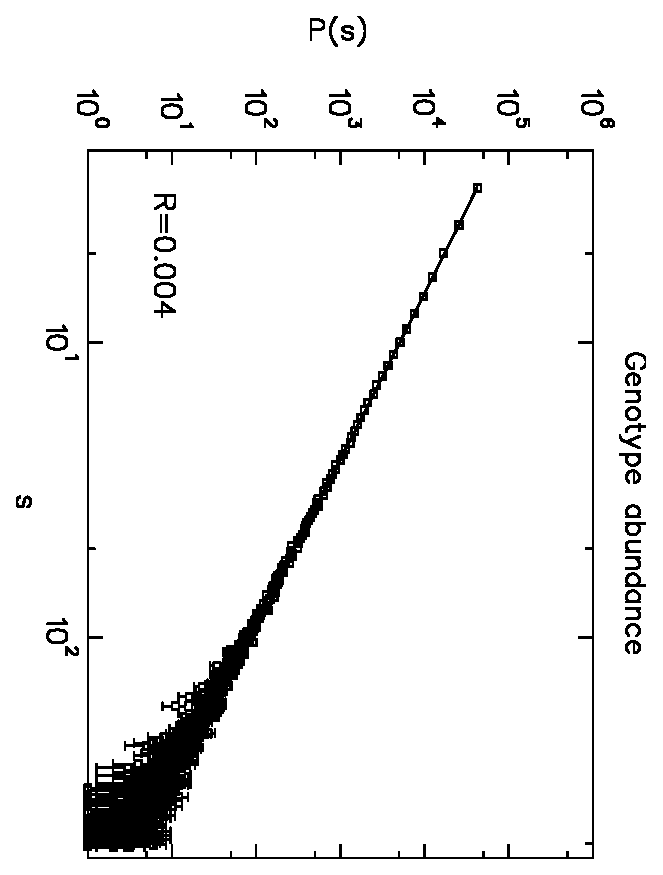
\includegraphics[width=2.25in, angle=90]{fig3.eps}
%\caption{Distribution of genotypes sizes $P(s)$ fitted to a power law
%  (solid line) at mutation rate $R=0.004$.}
%\label{fig3}
%\end{center}
%\end{figure}
%
%
%As mentioned earlier, we can also turn {\em off} all bonuses listed in
%Tab.~1, in which case fitness is related to replicative abilities
%only. Still, avalanches occur (within the first 50,000 updates
%monitored) due to minute improvements in fitness, but the length of
%the genomes typically stays in the range of the ancestor, a program of
%length 31 instructions. We expect a change of dynamics once the
%``true'' maximum of the local fitness landscape is reached, however,
%we did not reach this regime in the experiments presented here. The
%distribution of genotype sizes for the flat landscape is depicted in
%Fig.~\ref{fig4}.
%
%
%\begin{figure}[!tbp]
%\begin{center}
%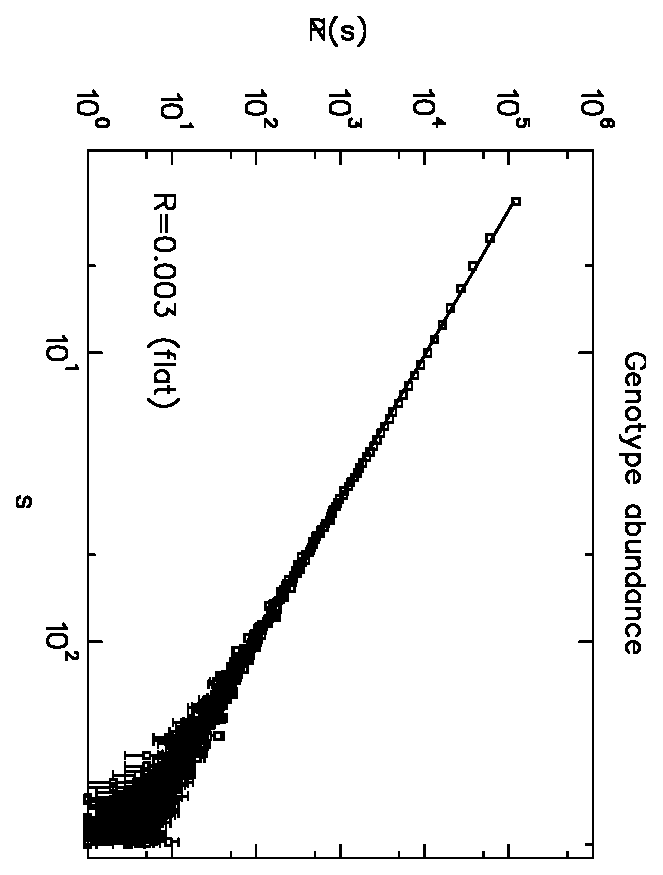
\includegraphics[width=2.25in, angle=90]{fig4.eps}
%\caption{Distribution of genotypes sizes $P(s)$ for a landscape devoid
%  of the bonuses listed in Tab.~1, at mutation rate $R=0.003$.} \label{fig4}
%\end{center}
%\end{figure}
%
%
%Clearly then, even such landscapes (flat with respect to all other
%activities except replication) are not neutral. Indeed, it is known
%that neutral evolution, where the chance for a genotype to increase or
%decrease in number is even, leads to a power law in the abundance
%distribution with exponent $D=1.5$ \citep{ABH}.
%
%
%\begin{figure}[t]
%\begin{center}
%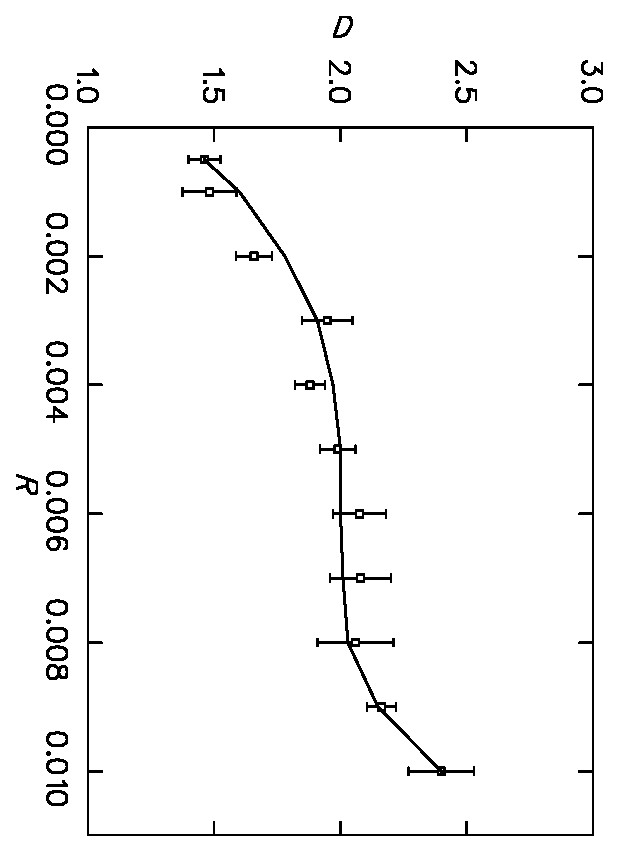
\includegraphics[width=2.2in, angle=90]{fig5.eps}
%\vskip 0.25cm
%\caption{Fitted exponent of power law for 34 runs at mutation rates
%  between $R=0.0005$ and $R=0.01$ copy errors per instruction
%  copied. The error bars reflect the standard deviation across the
%  sample of runs taken at each mutation rate. The solid line is to
%  guide the eye only.
%}
%\label{fig5}
%\end{center}
%\end{figure}
%
%
%In order to test the dependence of the fitted exponent $D(R)$
%[Eq.~(\ref{power})] on the mutation rate, we conduct a set of
%experiments at varying copy-mutation rates from $0.5\times10^{-3}$ to
%$10\times10^{-3}$ and take data for 50,000 updates. Again, a ``best''
%genotype is not reached after this time, and we must assume that
%avalanches were still occurring at the end of these runs. Furthermore,
%in some runs we find that a genotype comes to dominate the population
%(usually after most `genes' have been discovered) which carries an
%unusual amount of junk instructions. As mentioned earlier, such
%species produce a distribution that is exponentially suppressed at
%large genotype sizes (data not shown). To avoid contamination from
%such species, we stop recording genotypes after a plateau of fitness
%was reached, i.e., if the population had discovered most of the
%bonuses. Furthermore, in order to minimize finite size effects on the
%determination of the critical exponent, we excluded from this fit all
%genotype abundances larger than 15, i.e., we only fitted the smallest
%abundances. Indeed, at larger mutation rates the higher abundances are
%contaminated by a pile-up effect due to the toroidal geometry, while
%at lower mutation rates a scale appears to enter which prevents
%scale-free behavior. We have not, as yet, been able to determine the
%origin of this scale.
%
%In the results reported here, we show the dependence of the fitted
%exponent $D$ as a function of the mutation rate $R$ used in the run,
%which, however, is a good measure of the mutation probability $P$ only
%at small $R$ and if the sequence length is not excessive. As a
%consequence, data points at large $R$, as well as runs where an
%excessive sequence length developed, carry a systematic error.
%
\end{document}
